\section{Exercise 7.13 Human voice analysis}

\begin{lstlisting}[caption={MATLAB script dft\_voice.m}, label={lst:dft_unknown_note}]

name = 'a_low.wav';
[f, nu_s] = audioread(name);
f = f(:,1);
N_s = length(f);
F = fft(f);
Power = abs(F).^2;
v_k = (0:N_s-1)' * nu_s/N_s;   
 

R = real(ifft(Power));              
L = round(nu_s/500) : round(nu_s/60); 
[~, i] = max(R(L+1));                
nu_0 = nu_s / L(i);
fprintf('Base frequency: %.1f Hz\n', nu_0)
env = 10.^movmean(log10(Power), round(nu_0*N_s/nu_s));

 
% Plot 
low = v_k <= 3000;
semilogy(v_k(low), Power(low))
hold on
semilogy(v_k(low), env(low), 'k', 'LineWidth', 1.5)
hold off
xlabel('Frequency (Hz)')
ylabel('Power |F|^2 (arb. units)')
title(['Power spectrum of ', name], 'Interpreter', 'none')
legend('|F|^2', 'envelope')

\end{lstlisting}


\begin{figure}[H]
    \centering
    
\includegraphics[width=1\linewidth]{Figures/a_low_spectrum.png}
    \caption{A low power spectrum}
    \label{fig:placeholder}
\end{figure}

\begin{figure}[H]
    \centering
    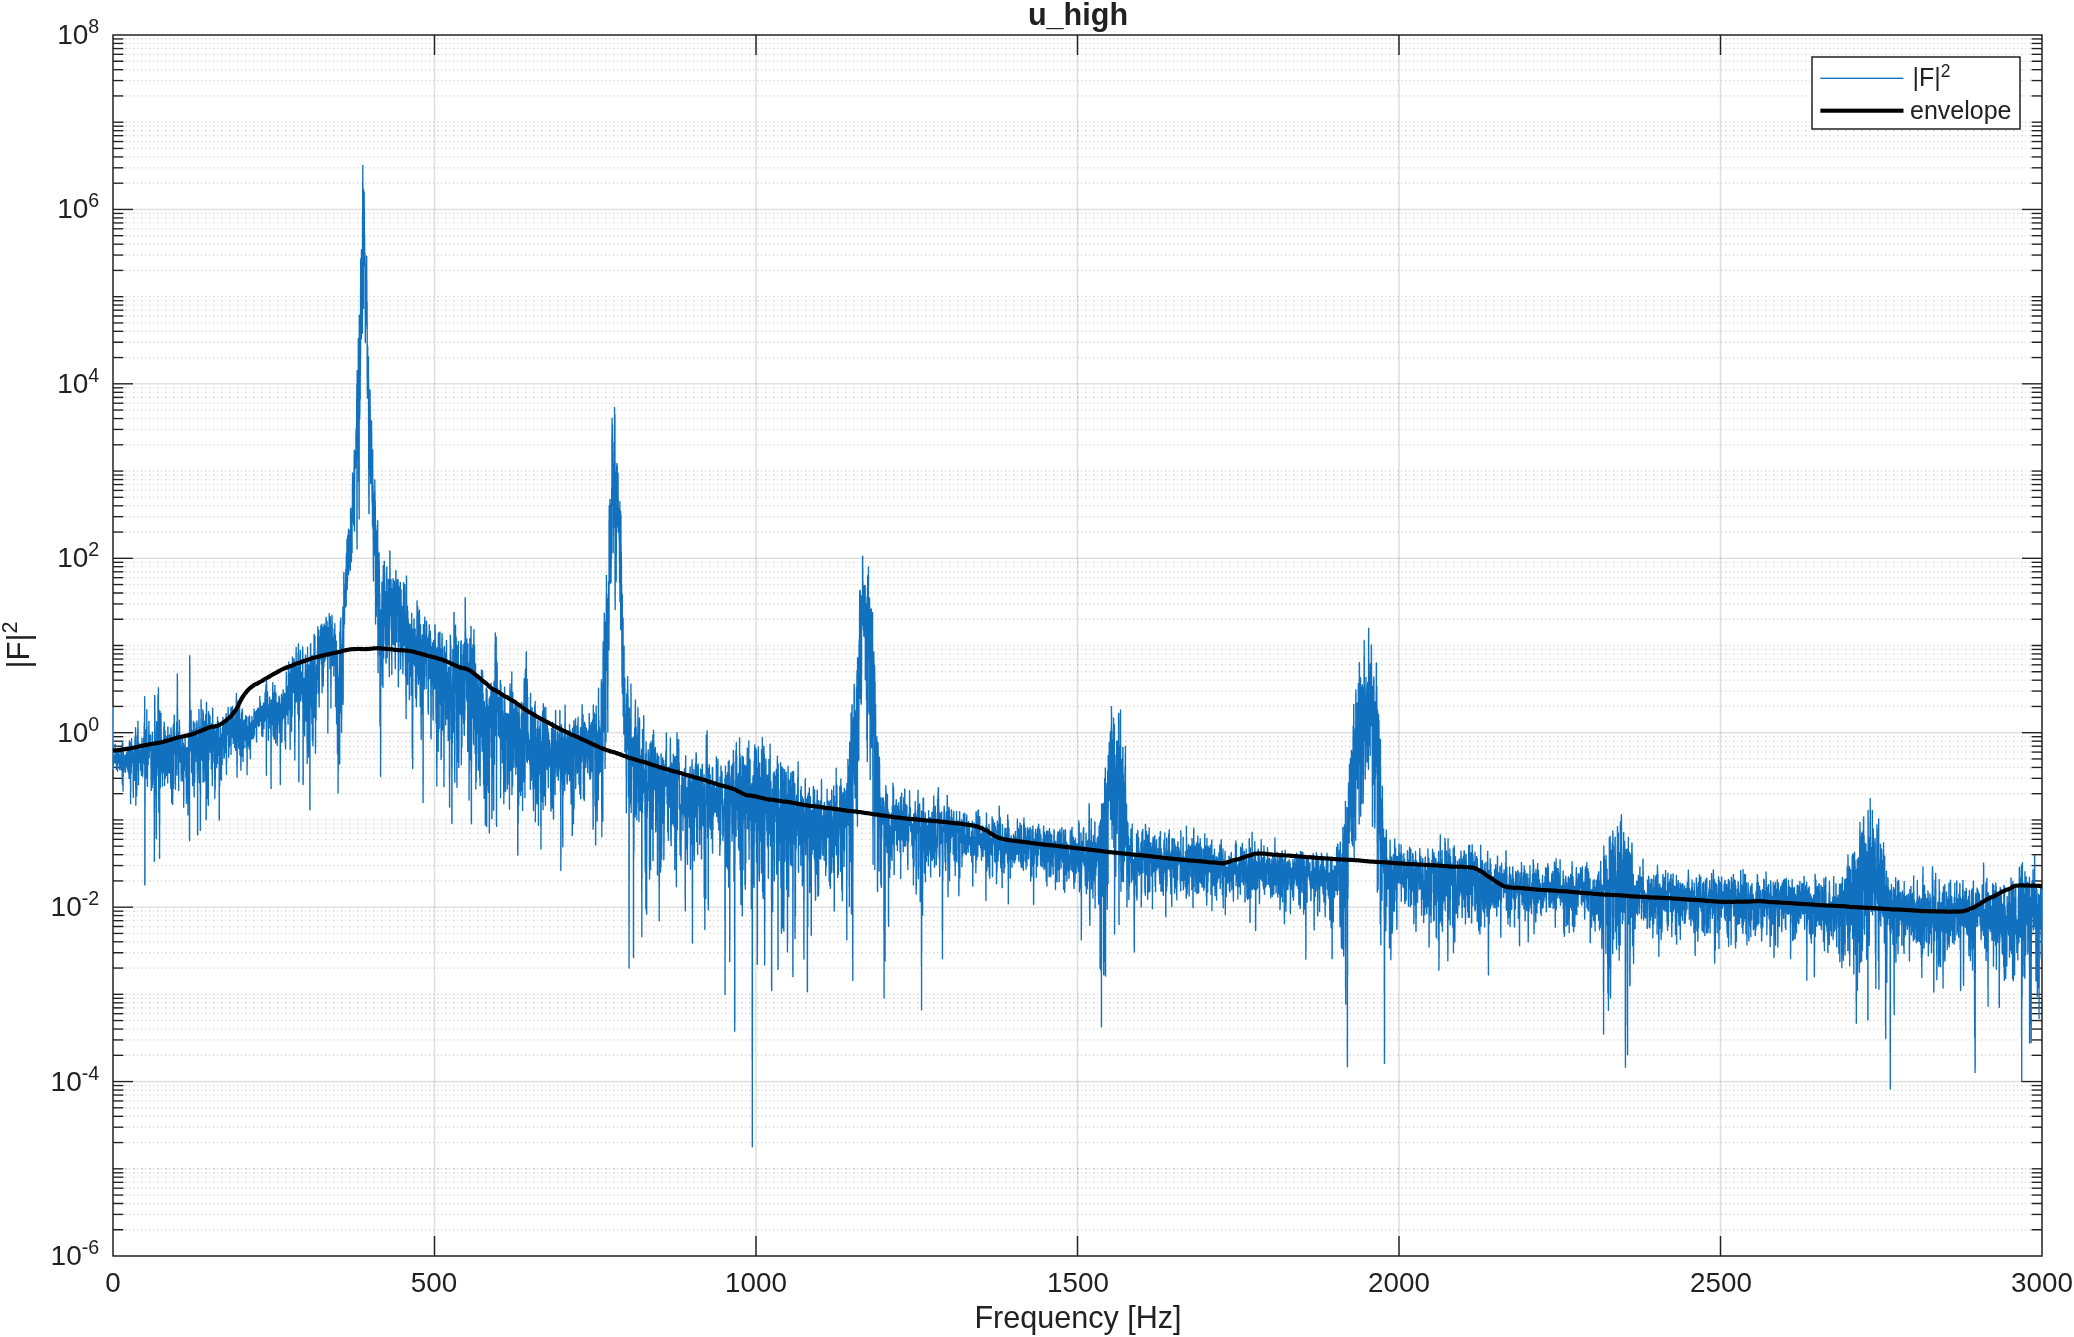
\includegraphics[width=1\linewidth]{Figures/u_high_spectrum.png}
    \caption{U high power spectrum}
    \label{fig:placeholder}
\end{figure}

\begin{figure}[H]
    \centering
    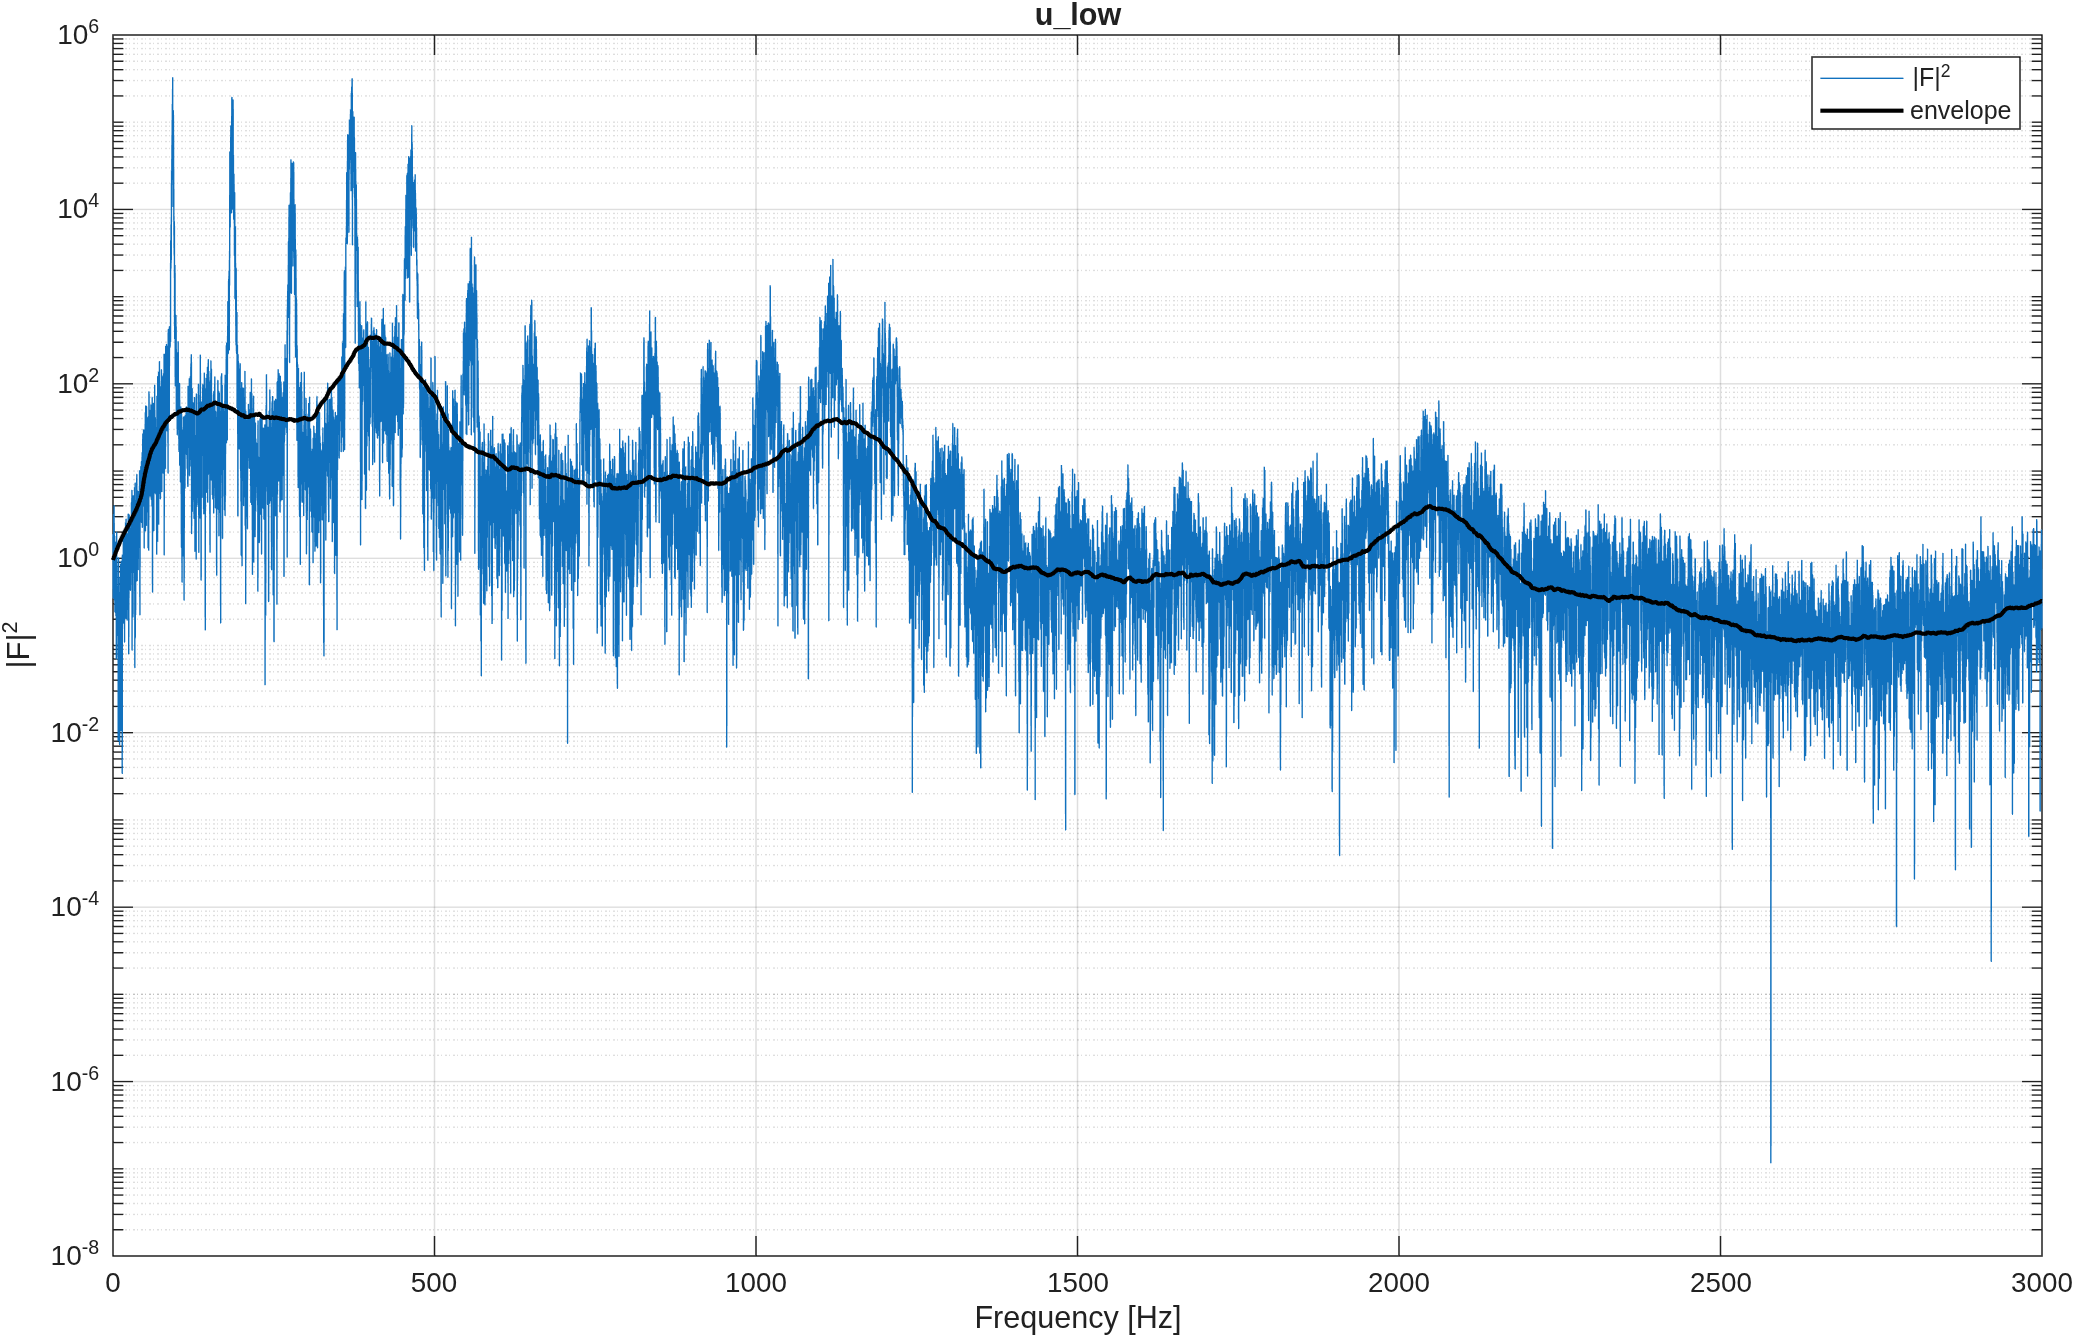
\includegraphics[width=1\linewidth]{Figures/u_low_spectrum.png}
    \caption{U low power spectrum}
    \label{fig:placeholder}
\end{figure}

\begin{table}[H]
    \centering
    \caption{Base frequencies for all voice recordings}
    \label{tab:placeholder}
    \renewcommand{\arraystretch}{1.2}
    \begin{tabular}{lc}
        \toprule
        A low   & 92.6 Hz \\
        U low   & 92.6 Hz \\
        U high  & 393.8 Hz \\
        \bottomrule
    \end{tabular}
\end{table}

\subsection*{Question 6: \texttt{u\_low.wav} compared with \texttt{u\_high.wav}}

\textbf{Base frequency.} The base frequency is not the same: $\nu_0 = 92.6$ Hz for \texttt{u\_low.wav} and $\nu_0 = 393.8$ Hz for \texttt{u\_high.wav}, about $4.3$ times higher (roughly two octaves).

\textbf{Formants.} The formants lie at the same frequencies. The first bump of the envelope is at about $400$ Hz in both spectra. For \texttt{u\_low.wav} the envelope also shows formants at about $1100$ Hz and $2050$ Hz. For \texttt{u\_high.wav} only the first one is visible in the envelope. This is because the harmonics lie at multiples of $\nu_0$, so they are $393.8$ Hz apart instead of $92.6$ Hz: below $3$ kHz there are only about $7$ harmonics against about $32$ for \texttt{u\_low.wav}, too few points to trace the shape of the envelope. The higher formant is still hinted at by the harmonic near $1950$ Hz, which is stronger than the one before it near $1560$ Hz, because it lies close to the formant at about $2050$ Hz.

\textbf{Is this expected?} Yes. The base frequency is set by the vibration of the vocal cords, which vibrate faster for the higher note. The formants are the resonance frequencies of the cavity formed by the throat and mouth, which depend only on its shape. Both recordings are the same vowel, so the cavity has the same shape and the formants stay in place. This matches the lecture notes (appendix D): when the base note is lower, the overtones lie closer together and the formants are better defined.

\subsection*{Question 7: \texttt{u\_low.wav} compared with \texttt{a\_low.wav}}

\textbf{Base frequency.} The base frequency is the same, $\nu_0 = 92.6$ Hz for both recordings. This can also be seen directly in the spectra: the spacing between neighbouring harmonics is the same in both.

\textbf{Formants.} The formants are at different frequencies. For \texttt{u\_low.wav} they are at about $400$, $1100$ and $2050$ Hz; for \texttt{a\_low.wav} at about $750$, $1200$ and $2550$ Hz. The first formant changes the most (it almost doubles), the second one only shifts slightly.

\textbf{Is this expected?} Yes. Both vowels were sung at the same low pitch, so the vocal cords vibrate at the same rate and $\nu_0$ is unchanged. Changing the vowel from ``u'' to ``a'' changes the shape of the cavity (the mouth opens and the tongue moves), which changes its resonance frequencies and therefore the formants. According to the lecture notes (appendix D), the first two formants $F_1$ and $F_2$ completely determine which vowel is produced.
